\documentclass{beamer}
\usepackage{hyperref}
\usepackage{color}
\usepackage{multirow} 
\usepackage{url}
\usepackage{verbatim}
%\usepackage{subfig}
%\usepackage{float}
%\DisemulatePackage{setspace}
%\usepackage{setspace}
%\usepackage[usenames,dvipsnames]{color}
\usetheme{Warsaw}

\useoutertheme{infolines}
\useinnertheme{rounded}
\setbeamercovered{dynamic}
\setbeamerfont{caption}{size=\scriptsize}
\setbeamercovered{dynamic}
\setlength{\abovecaptionskip}{-0.5ex}
\setlength{\belowcaptionskip}{-2ex}
%\setbeamercolor*{palette primary}{use=structure,fg=white,bg=blue!60}
%\setbeamercolor*{palette quaternary}{fg=white,bg=blue!30!black}
\setbeamercolor*{palette primary}{use=structure,fg=white,bg=gray!60}
\setbeamercolor*{palette quaternary}{fg=white,bg=gray!30!black}
\newcommand{\removepagenumbers}{% 
  \setbeamertemplate{footline}{ 
     \leavevmode% 
     \hbox{% 
     \begin{beamercolorbox}[wd=.333333\paperwidth,ht=2.25ex,dp=1ex,center]{author in head/foot}% 
        \usebeamerfont{author in head/foot}\insertshortauthor~~(\insertshortinstitute) 
     \end{beamercolorbox}% 
     \begin{beamercolorbox}[wd=.333333\paperwidth,ht=2.25ex,dp=1ex,center]{title in head/foot}% 
       \usebeamerfont{title in head/foot}\insertshorttitle 
     \end{beamercolorbox}% 
     \begin{beamercolorbox}[wd=.333333\paperwidth,ht=2.25ex,dp=1ex,right]{date in head/foot}% 
       \usebeamerfont{date in head/foot}\insertshortdate{}\hspace*{2em} 
%    \insertframenumber{} / \inserttotalframenumber\hspace*{2ex} 
     \end{beamercolorbox}}% 
     \vskip0pt% 
   }% 
} 



%\thispagestyle{empty}
\title[Compensator design for active analog circuit]{COMPENSATOR DESIGN FOR ACTIVE ANALOG CIRCUIT}
\author[]{Presented by \\
{\Large \bf {Shalini Shrivastava}} \\
%\vspace{0.5cm}
Under the guidance of\\
{\bf Prof. V.R.Sule and Prof. M.S.Baghini}}
\institute[{\url{shalini@ee.iitb.ac.in}}]{\includegraphics[scale=0.15]{images/iitblogo}\\
\bf{Department  of Electrical Engineering\\
Indian Institute of Technology, Bombay}}
\date{M.Tech. First stage}




\AtBeginSection[]
{

{\removepagenumbers
   \begin{frame}
       \frametitle{Compensation Design For Active Analog Circuit}
\addtocounter{framenumber}{-1}
       \tableofcontents[currentsection]
   \end{frame}
}
}

\begin{document}
{\removepagenumbers
\begin{frame}
\addtocounter{framenumber}{-1}
\titlepage
\end{frame}
}



%%%%TITLE

\begin{frame}
\frametitle{Compensation Design for Active Analog Circuit}
\tableofcontents
\end{frame}

%%%%MOTIVATION 1

\section{Introduction}
\subsection*{Motivation}
\begin{frame}
\frametitle{Motivation \& Introduction}
\begin{small}

\begin{itemize}
        \item{Active network, under certain circumstances, may become unstable and therefore break into oscillation.}
	\item{As technology is scaling down,and require high speed and low power consumption, the main issue is the stability of complete circuit.}
        \item{Existing graphical approach does not provide the compensation network, While with coprime factorization approach using state space gives set of compensators.}
        \item{State space is the modern approach, which enables to shortcomings of transfer function approach \cite{Mitra}.}
        \item{State-space description of a network or system emphasizes the internal structure of that system, as well as its input-output performance \cite{Ander}, used in analysis and synthesis of the system.}
 \end{itemize}
	\end{small}
\let\thefootnote\relax\footnotetext[\value{footnote}]{\tiny{{{{~\cite{Mitra}\color{blue}Sanjit Kumar Mitra, Analysis and Synthesis of Linear Active Networks, John Wiley and Sons, Inc,1969.}}}}\\{{{~\cite{Ander}\color{blue}B.D.O. Anderson and S. Vongpanitlerd, Network analysis and synthesis: a modern
systems theory approach, Courier Dover Publications, 2006.}}}}	
\end{frame}
%%%%{\hyperlink{Survey}{\beamergotobutton{3}}}{\hyperlink{2necessary}{\beamergotobutton{3}}}
%%%%%%%%%%%%%%%%%%%% Second 


%%%%MOTIVATION 2 

\subsection*{Motivation}
\begin{frame}
\frametitle{Motivation \& Introduction}
\begin{small}

\begin{figure}
	\begin{center}
	
        \includegraphics[scale=0.25,angle=360]{./images/SAVE}
 		%\caption{One Port Network.}
        \label{save}
	\end{center}
	\end{figure}
	\end{small}
\end{frame}


%%%%%%%%%%%%%%%%%%%%%%%%%%%%%% 3

\section{Stability}

\subsection*{Stability}

\begin{frame}
\frametitle{Stability}

\begin{small}
        \begin{itemize}
	\item{Network is said to be stable if as a result of subjecting it to an excitation which dies out with time, the response remains bounded in amplitude as time grows indefinitely \cite{Haykin}.}
\item{Open circuit stability test: Network is said to be open circuit stable, when poles of driving point impedance lies in left half of s-plane. For open circuit unstable network, compensator is to be connected in parallel with given circuit}
\item{Short circuit stability test: Network is said to be short circuit stable, when poles of driving point admittance lies in left half of s-plane. For short circuit unstable network, compensator is to be connected in series with given circuit.}
                \end{itemize}
\end{small}
\let\thefootnote\relax\footnotetext[\value{footnote}]{\tiny{{{~\cite{Haykin}\color{blue}S.S.Haykin, Active Network Theory, Addison-Wesley Publishing Company, 1970.}}}}	
\end{frame}





%%%%%%%%%%%%%%%%%%%%%%%%%%% 4



\subsection*{Compensator Design}

\begin{frame}
\frametitle{Compensator Design}

\begin{small}
        \begin{itemize}
	\item Let one port network is specified by its minimal driving point impedance z(s)
\begin{equation}
z(s)=\frac{n(s)}{d(s)}
\end{equation}
 where n(s) and d(s) are coprime.
        \item By Euclidean algorithm, it is possible to obtain two polynomials x(s) \& y(s) satisfying Bezout identity:
\begin{equation}
n(s)x(s)+d(s)y(s)=1
\end{equation}
 where controller impedance is $z_c(s)=\frac{y(s)}{x(s)}$
\item It may be possible that x(s) may be zero, for which controller is undefined.
\item The solution to overcome this problem is to arrange these four polynomials n(s), d(s), x(s) and y(s) as rational expressions as elements of $\wp$  which represents the family of all stable, proper and real rational functions \cite{Doyle}.
\end{itemize}
\end{small}
\let\thefootnote\relax\footnotetext[\value{footnote}]{\tiny{{{~\cite{Doyle}\color{blue}John C. Doyle, Bruce A. Francis, Allen R. Tannenbaum, Feedback Control Theory, Dover Publications, Inc. Mineola, New York, 2009.}}}}	
\end{frame}
	



%%%%%%%%%%%%%%%%%%%%%%%%%%% 6 



\subsection*{Coprime Factorization}

\begin{frame}
\frametitle{Coprime Factorization}

\begin{small}
        \begin{itemize}
	\item N(s), D(s), X(s) and Y(s) as elements of $\wp$ instead of polynomials.
         \item Let Z(s) be impedance function of one port network given as,
\begin{equation}
Z(s)=\frac{N(s)}{D(s)}
\end{equation}

        \item By Euclidean algorithm, it is possible to obtain two polynomials X(s) \& Y(s) satisfying Bezout identity:
\begin{equation}
N(s)X(s)+D(s)Y(s)=1
\end{equation}
where, N(s), D(s) $\in$ $\wp$ and are coprime. This is called coprime factorization of Z(s) over $\wp$.
\item It is required to get N(s),D(s), X(s) and Y(s), all in $\wp$ using state space method. 
%% \item Obtain N(s),D(s), X(s) and Y(s).
\item Let the input and output of Z(s) be denoted as u and y respectively. Then the state model of Z(s) is given as, $\dot{x}=Ax+Bu$ and y=Cx+du. 
\end{itemize}
\end{small}
%%%%%%%\let\thefootnote\relax\footnotetext[\value{footnote}]{\tiny{{{~\cite{Haykin}\color{blue}S.S.Haykin, Active Network Theory, Addison-Wesley Publishing Company, 1970.}}}}	
\end{frame}
%%%%%%%%%%%%%%%%%%%%%%%%%%%%%%%%





\subsection*{Coprime Factorization}

\begin{frame}
\frametitle{Coprime Factorization}

\begin{small}
        \begin{itemize}
\item Now choose a real matrix F, $1 \times n$, such that A + BF is stable i.e. all the eigenvalues in Re $s < 0$.
\item Define a signal v:= u – Fx ⟹ u = Fx + v. Substituting this in above state model we get,
\begin{equation}
\dot{x}=(A+BF)x+Bv; \hspace{.5in} y=(C+DF)x+Dv
\end{equation}
\item The transfer function from v to u is given by, 
\begin{equation}
D(s)=1+F[sI-(A+BF)]^{-1}B
\end{equation}
\item The transfer function from v to y is given by, 
\begin{equation}
N(s)=D+(C+DF)[sI-(A+BF)]^{-1}B
\end{equation}

\item Similarly, choose a real matrix H, $n \times 1$, such that A + HC is stable i.e. all the eigenvalues in Re $ s < 0$.
\begin{equation}
X(s)=F[sI-(A+HC)]^{-1}H
\end{equation}
\begin{equation}
Y(s)=1+F[sI-(A+BF)]^{-1}(-B-HD)
\end{equation}
\end{itemize}
\end{small}
%%%%%%%%\let\thefootnote\relax\footnotetext[\value{footnote}]{\tiny{{{~\cite{Haykin}\color{blue}S.S.Haykin, Active Network Theory, Addison-Wesley Publishing Company, 1970.}}}}	
\end{frame}

%%%%%%%%%%%%%%%55

\subsection*{Compensator}

\begin{frame}
\frametitle{Compensator }

\begin{small}
        \begin{itemize}
	\item Theorem: If Z(s)=$\frac{N(s)}{D(s)}$ be a coprime factorization over $\wp$ with X(s) and Y(s) be two functions in $\wp$ satisfying the equation N(s)X(s)+D(s)Y(s)=1, then the set of all compensators that can stabilize Z is given by,
\begin{equation}
Z_c(s)=\frac{Y(s)-N(s)Q}{X(s)+D(s)Q}
\end{equation}
 where Q $\in \wp$, known as free parameter.
\end{itemize}
\end{small}
%%%\let\thefootnote\relax\footnotetext[\value{footnote}]{\tiny{{{}}}}	
\end{frame}
	



%%%%%%%%%%%%%%%%%%%%%%%%%%% 6 


%%%%%%%%%%%%%%%%%%%%%%%%%%Flow
\section{State Space}
\subsection*{Formulation}

\begin{frame}
\frametitle{Algorithm}

\begin{small}
\begin{figure}
	\begin{center}
	
        \includegraphics[scale=0.4,angle=360]{./images/flow}
 		%%\caption{One Port Network.}
        \label{flowA}
	\end{center}
	\end{figure}

\end{small}
\end{frame}

%%%%%%%%%%%%%%%%%%%%%%%%% 9

\subsection*{Formulation}

\begin{frame}
\frametitle{Example}
\begin{small}
        \begin{itemize}
\item {Figure \ref{ex3} (a) shows a circuit model of a transistor tuned amplifier based on the y-parameter model of the transistor.Develop state-space equation for circuit. Assume first that $Y_{12}$ and $Y_{21}$ and real constant. Example is unsolved example of \cite{Ander}.}

\begin{figure}[h!]
\centering
{\label{method}\includegraphics[totalheight=.2\textheight,width=.6\textwidth]{images/Trans}}
%\subfloat[]{\label{mlfsr}\includegraphics[totalheight=.3\textheight,width=.3\textwidth]{images/LowFreqMag.png}}
\caption{Example 2}
\label{ex3}
\end{figure} 

\end{itemize}
\end{small}

\let\thefootnote\relax\footnotetext[\value{footnote}]{\tiny{{{~\cite{Ander}\color{blue}B.D.O. Anderson and S. Vongpanitlerd, Network analysis and synthesis: a modern
systems theory approach, Courier Dover Publications, 2006.}}}}	

%%%%{\hyperlink{Survey}{\beamergotobutton{3}}}{\hyperlink{2necessary}{\beamergotobutton{3}}}
\end{frame}




%%%%%%%%%Step 1
\subsection*{Formulation}

\begin{frame}
\frametitle{Example}
\begin{small}
\begin{itemize}
\item Step 1: Write the state space equation of the given network in the form of A $(3 \times 3)$, B$(3 \times 1)$, C$(1 \times 3)$, D $(1 \times 1)$ matrices with input $[V]$, output voltage $ [V_o]$, and state variables as $x=[V_{c1} \hspace{.2in} V_{c2} \hspace{.2in}I_l]^T$.\\

State Space equations are:
\[ \left[ \begin{array}{cc}
\dot{V_{c1}} \\
\dot{V_{c2}} \\
\dot{I_l}
\end{array} \right]
=
\left[ \begin{array}{ccc}
A_{11} & A_{12} & A_{13}\\
A_{21} & A_{22} & A_{23}\\
A_{31} & A_{32} & A_{33}
\end{array} \right]
%
\left[ \begin{array}{c}
{V_{c1}} \\
{V_{c2}} \\
{I_l}
\end{array} \right]
+
\left[ \begin{array}{c}
B_{11} \\
B_{21} \\
B_{31}
\end{array} \right]
%
\left[ \begin{array}{c}
{V}
\end{array} \right]
\]
Output equation:
\[ \left[ \begin{array}{c}
{V_o} 
\end{array} \right]
=
\left[ \begin{array}{ccc}
C_{11} & C_{12} & C_{13}
\end{array} \right]
%
\left[ \begin{array}{cc}
{V_{c1}} \\
{V_{c2}}\\
{I_l}
\end{array} \right]
+
\left[ \begin{array}{cc}
D
\end{array} \right]
%
\left[ \begin{array}{cc}
{V}
\end{array} \right]
\]

\end{itemize}
\end{small}
\end{frame}


%%%%%%%%%Step 2
\subsection*{Formulation}

\begin{frame}
\frametitle{Example}
\begin{small}
\begin{itemize}
\item Step 2: Make input $V$ as zero, i.e. voltage source (V) should be short, as shown in Fig. \ref{transa}. And Substitute Inductor by current source $I_l$ and Capacitors by voltage source $V_{c1}$ \& $V_{c2}$

\begin{figure}[h!]
\centering
{\label{method}\includegraphics[totalheight=.2\textheight,width=.6\textwidth]{images/Transa}}
%\subfloat[]{\label{mlfsr}\includegraphics[totalheight=.3\textheight,width=.3\textwidth]{images/LowFreqMag.png}}
\caption{Step 2}
\label{transa}
\end{figure} 

\item Step 3: As here we have two sources we will use the superposition theorem to find the coefficient of matrix [A] and [C]
%Matrix A
\begin{itemize}
\item{Let $V_{c2}$ and $I_l=0$, State space equation become as:} \\

\[ \left[ \begin{array}{cc}
\dot{V_{c1}} \\
\dot{V_{c2}} \\
\dot{I_l}
\end{array} \right]
=
\left[ \begin{array}{ccc}
A_{11} \\
A_{21} \\
A_{31} 
\end{array} \right]
%
\left[ \begin{array}{c}
{V_{c1}}
\end{array} \right];
\left[ \begin{array}{c}
{V_{o}}
\end{array} \right]
=
\left[ \begin{array}{c}
{C_{11}}
\end{array} \right]
\left[ \begin{array}{c}
{V_{c1}}
\end{array} \right]
\]
\end{itemize}
\end{itemize}
\end{small}
\end{frame}


%%%%%%%%%%%%%%%%% A1 C1
\subsection*{Formulation}

\begin{frame}
\frametitle{Example}
\begin{small}
\begin{itemize}
\item Calculate $I_{c1}$ in terms of $V_{c1}$\\
\begin{equation}
I_{c1}=\frac{1}{(R_1||R_2)}V_{c1};\hspace{.3in} \dot{V}_{c1}=\frac{(R_1+R_2)}{C_1R_1R_2}V_{c1};\hspace{.3in} A_{11}=\frac{(R_1+R_2)}{C_1R_1R_2}
\end{equation}

\item Calculate $I_{c2}$ in terms of $V_{c1}$\\
\begin{equation}
I_{c2}=-Y_{21}V_{R};\hspace{.3in} \dot{V}_{c1}=-\frac{Y_{21}}{C_2}V_{c1};\hspace{.3in} A_{12}=-\frac{Y_{21}}{C_2}
\end{equation}
\item Calculate $V_{l}$ in terms of $V_{c1}$\\
\begin{equation}
V_{l}=0;\hspace{.3in} \dot{I}_{l}=0V_{c1} \hspace{.3in} A_{13}=0
\end{equation}
\item Calculate $V_{o}$ in terms of $V_{c1}$\\
\begin{equation}
V_o=0; \hspace{0.3in} C_{11}=0
\end{equation}
\end{itemize}
\end{small}
\end{frame}


%%%%%%%%%%%%%%%%% A2 C2
\subsection*{Formulation}

\begin{frame}
\frametitle{Example}
\begin{small}
\begin{itemize}
\item{Let $V_{c1}=0$ and $I_l=0$, State space equation become as:} \\

\[ \left[ \begin{array}{cc}
\dot{V_{c1}} \\
\dot{V_{c2}} \\
\dot{I_l}
\end{array} \right]
=
\left[ \begin{array}{ccc}
A_{21} \\
A_{22} \\
A_{32} 
\end{array} \right]
%
\left[ \begin{array}{c}
{V_{c2}}
\end{array} \right];
\left[ \begin{array}{c}
{V_{o}}
\end{array} \right]
=
\left[ \begin{array}{c}
{C_{12}}
\end{array} \right]
\left[ \begin{array}{c}
{V_{c2}}
\end{array} \right]
\]
\item Calculate $I_{c1}$ in terms of $V_{c2}$\\
\begin{equation}
I_{c1}=-Y_{12}V_{o};\hspace{.3in} \dot{V}_{c1}=-\frac{Y_{12}}{C_1}V_{c2};\hspace{.3in} A_{21}=-\frac{Y_{12}}{C_1}
\end{equation}

\item Calculate $I_{c2}$ in terms of $V_{c2}$\\
\begin{equation}
I_{c2}=\frac{1}{R_3}V_{c2};\hspace{.3in} \dot{V}_{c2}=\frac{1}{R_3C_2}V_{c2};\hspace{.3in} A_{22}=\frac{1}{R_3C_2}
\end{equation}
\item Calculate $V_{l}$ in terms of $V_{c2}$\\
\begin{equation}
V_{l}=V_{c2};\hspace{.3in} \dot{I}_{l}=\frac{1}{L}V_{c2} \hspace{.3in} A_{32}=\frac{1}{L}
\end{equation}

\end{itemize}
\end{small}
\end{frame}
%%%%%%%%%%%%%%%%%%%%%%A3 C#
\subsection*{Formulation}

\begin{frame}
\frametitle{Example}
\begin{small}
\begin{itemize}
\item Calculate $V_{o}$ in terms of $V_{c2}$\\
\begin{equation}
V_o=V_{c2}; \hspace{0.3in} C_{12}=1
\end{equation}
\item{Let $V_{c1}=0$ and $V_{c2}=0$, State space equation become as:} \\

\[ \left[ \begin{array}{cc}
\dot{V_{c1}} \\
\dot{V_{c2}} \\
\dot{I_l}
\end{array} \right]
=
\left[ \begin{array}{ccc}
A_{31} \\
A_{32} \\
A_{33} 
\end{array} \right]
%
\left[ \begin{array}{c}
{I_l}
\end{array} \right];
\left[ \begin{array}{c}
{V_{o}}
\end{array} \right]
=
\left[ \begin{array}{c}
{C_{13}}
\end{array} \right]
\left[ \begin{array}{c}
{I_l}
\end{array} \right]
\]

\item Calculate $I_{c1}$ in terms of $I_l$\\
\begin{equation}
I_{c1}=-Y_{12}V_{o}; \hspace{.3in}I_{c1}=0;\hspace{.3in} \dot{V}_{c1}=0I_l;\hspace{.3in} A_{31}=0
\end{equation}

\item Calculate $I_{c2}$ in terms of $I_l$\\
\begin{equation}
I_{c2}=-I_l;\hspace{.3in} \dot{V}_{c2}=-\frac{1}{C_2}I_{l};\hspace{.3in} A_{32}=\frac{1}{C_2}
\end{equation}

%\end{equation}
\end{itemize}
\end{small}
\end{frame}

%%%%%%%%%%%%%%%%%%%%%%%A3
\subsection*{Formulation}

\begin{frame}
\frametitle{Example}
\begin{small}
\begin{itemize}
\item Calculate $V_{l}$ in terms of $I_l$\\
\begin{equation}
V_{l}=0;\hspace{.3in} \dot{I}_{l}=0I_l; \hspace{.3in} A_{33}=0
\end{equation}

\item Calculate $V_{o}$ in terms of $I_l$\\
\begin{equation}
V_o=0; \hspace{0.3in} C_{13}=0
\end{equation}
\end{itemize}
\end{small}
\end{frame}

%%%%%%%%%%%%%%%%%%%%%%BBBBBBBBBBBBBBB

\subsection*{Formulation}

\begin{frame}
\frametitle{Example}
\begin{small}

\begin{itemize}
\item Step 5: Make state variable x zero, i.e. capacitor should be short, and inductor open circuit as shown in Fig. \ref{transb}.

\begin{figure}[h!]
\centering
{\label{method}\includegraphics[totalheight=.2\textheight,width=.6\textwidth]{images/Transc}}
%\subfloat[]{\label{mlfsr}\includegraphics[totalheight=.3\textheight,width=.3\textwidth]{images/LowFreqMag.png}}
\caption{Step 2}
\label{transb}
\end{figure} 

State Space equations are:
\[ \left[ \begin{array}{cc}
\dot{V_{c1}} \\
\dot{V_{c2}} \\
\dot{I_l}
\end{array} \right]
=
\left[ \begin{array}{c}
B_{11} \\
B_{21} \\
B_{31}
\end{array} \right]
%
\left[ \begin{array}{c}
{V}
\end{array} \right]; \hspace{0.3in}
 \left[ \begin{array}{c}
{V_o} 
\end{array} \right]
=
\left[ \begin{array}{cc}
D
\end{array} \right]
%
\left[ \begin{array}{cc}
{V}
\end{array} \right]
\]
%\end{itemize}
\end{itemize}
\end{small}
\end{frame}

%%%%%%%%%%%%%%%%% BBBBBDDDDDDD
\subsection*{Formulation}

\begin{frame}
\frametitle{Example}
\begin{small}
\begin{itemize}
\item Calculate $I_{c1}$ in terms of $V$\\
\begin{equation}
I_{c1}=-\frac{1}{R_1}V;\hspace{.3in} \dot{V}_{c1}=-\frac{1}{C_1R_1}V;\hspace{.3in} B_{11}=-\frac{1}{C_1R_1}
\end{equation}

\item Calculate $I_{c2}$ in terms of $V$\\
\begin{equation}
I_{c2}=-Y_{12}V_{R};\hspace{.3in} \dot{V}_{c1}=0 V;\hspace{.3in} B_{12}=0
\end{equation}
\item Calculate $V_{l}$ in terms of $V$\\
\begin{equation}
V_{l}=0;\hspace{.3in} \dot{I}_{l}=0V \hspace{.3in} B_{13}=0
\end{equation}
\item Calculate $V_{o}$ in terms of $V$\\
\begin{equation}
V_o=0; \hspace{0.3in} D=0
\end{equation}
\end{itemize}
\end{small}
\end{frame}

%\end{document}




%%%%%%%%%State Space
\subsection*{Formulation}

\begin{frame}
\frametitle{Example}
\begin{small}
\begin{itemize}
\item State Space equations are:

\[ \left[ \begin{array}{cc}
\dot{V_{c1}} \\ \dot{V_{c2}} \\ \dot{I_l}
\end{array} \right]
=
\left[ \begin{array}{ccc}
\frac{R_1+R_2}{C_1R_1R_2} & -\frac{Y_{12}}{C_2} & 0\\
-\frac{Y_21}{C1} & \frac{1}{R_3C_2} & \frac{1}{C_2}\\
0 & \frac{1}{L}& 0
\end{array} \right]
%
\left[ \begin{array}{c}
{V_{c1}} \\
{V_{c2}} \\
{I_l}
\end{array} \right]
+
\left[ \begin{array}{c}
-\frac{1}{R_1C_1} \\
0 \\
0
\end{array} \right]
%
\left[ \begin{array}{c}
{V}
\end{array} \right]
\]
Output equation:
\[ \left[ \begin{array}{c}
{V_o} 
\end{array} \right]
=
\left[ \begin{array}{ccc}
0 & 1 & 0
\end{array} \right]
%
\left[ \begin{array}{cc}
{V_{c1}} \\
{V_{c2}}\\
{I_l}
\end{array} \right]
+
\left[ \begin{array}{cc}
0
\end{array} \right]
%
\left[ \begin{array}{cc}
{V}
\end{array} \right]
\]

%\item Transfer Function is given as:\\
%$TF=B(SI-A)^(-1)C+D$
\end{itemize}
\end{small}
\end{frame}


%%%%%%%%%%%%%%%%%%%Limiations
%\section{Compensation Design Example}
\subsection*{Formulation}

\begin{frame}
\frametitle{Limitations}

\begin{small}
       \begin{itemize}
          \item Circuit should have finite components \& finite number of controlled sources.
          \item The network does not contain a node with the only elements incident at node comprising
inductor and/or current generator. i.e the network does not contain a cut set.
          \item The network does not contain a loop with the only branches in the loop comprising capacitor
and/or voltage generator. i.e. the network does not contain a tie set.
          %\item
       \end{itemize}
\end{small}
\end{frame}

%%%%%%%%%%%%%%%%%%%%%%%%% 1000
\section{Example}
\subsection*{Example}

\begin{frame}
\frametitle{Example}

\begin{small}
        \begin{itemize}
	\item{In this section we summarized the whole research work with an  example.
The circuit of Fig.\ref{ex2} is a first-order circuit with voltage controlled current source, taken from unsolved example of \cite{Chua}.
\begin{figure}[h!]
\centering
{\label{method}\includegraphics[totalheight=.2\textheight,width=.6\textwidth]{images/ex3a}}
%\subfloat[]{\label{fig:eyediagram}\includegraphics[width=0.6\textwidth]{images/ex3b}}\\
%\subfloat[]{\label{fig:eyediagram}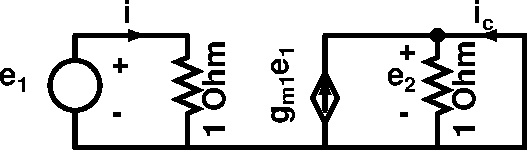
\includegraphics[width=0.6\textwidth]{images/ex3c}}
%\caption{(a) Block diagram of testing of DAC with PRBS. (b) Eyediagram for the 4-bit DAC output with 6-bit PRBS and (c) 
% Eyediagram for the 4-bit DAC output with 8-bit PRBS }
\caption{Example to find the Compensator}
\label{ex3a}
\end{figure}}



         \end{itemize}
\end{small}

\let\thefootnote\relax\footnotetext[\value{footnote}]{\tiny{{{~\cite{Chua}\color{blue}L.O.Chua, C.A.Deoser and E.H.Kuh, Linear and Nonlinear Circuits. New York: Mcgraw-Hill,1987}}}}	

\end{frame}



%%%%%%%%%%%%%%%%%%%%%%%%% 1000
%%%%%%%%%%%%%%%%%%%%%%%%% 1000
%%%%%%%%%%%\section{Compensation Design Example}
\subsection*{state space}

\begin{frame}
\frametitle{Example}

\begin{small}
        \begin{itemize}
	\item Step 1: Write the state space equation of the given network in the form of A, B, C, D matrices with x as $V_c$, u input as $ e_1$ voltage and y as output current $ i$.
\begin{equation}
 [\dot{V}_c]=[A][V_c]+[B][e_1]
\end{equation}
\begin{equation}
 [i]=[C][V_c]+[D][e_{1}]
\end{equation}
\item Step 2: Make input $e_1$ as zero, i.e. voltage source should be short, and substitute capacitor with voltage source of $V_c$ as shown in Fig. \ref{ex2}.


\begin{figure}[h!]
\centering
{\label{method}\includegraphics[totalheight=.2\textheight,width=.6\textwidth]{images/ex3b}}
\caption{Input=0}
\label{ex2}
\end{figure}


\item State space equation modified as:\\
\begin{equation}
 [\dot{V}_c]=[A][V_c]; \hspace{.2in}[i]=[C][V_c]
\end{equation}
         \end{itemize}
\end{small}


\end{frame}




%%%%%%%%%%%%%%%%%%%%%%%%% 1000
%%%%%%%%%%%%%%%%%%%%%%%%% 1000
%%%%%%%%%%%\section{Compensation Design Example}
\subsection*{Example}

\begin{frame}
\frametitle{Example}

\begin{small}
        \begin{itemize}
	\item Step 3: Calculate $ I_c$ in terms of $V_c$. 
\begin{equation}
I_c=V_c; \hspace{0.2in} C\dot{V}_c=V_c;\hspace{0.2in}\dot{V}_c=\frac{1}{C}V_c;\hspace{0.2in} [A]=1
\end{equation}
         \item Step 4:Determine the output $i$ in terms of state variable$V_c$.
\begin{equation}
i=-g_{m2}e_2; \hspace{0.2in}e_2=V_c; \hspace{0.2in} i=-g_{m2}V_c \hspace{0.2in} i=-2V_c;\hspace{0.2in}[C]=-2
\end{equation}
\item Step 5: Short circuits the capacitor to make state variable x=0 in original circuit and Redraw the circuit shown in Fig.\ref{ex3c}.

\begin{figure}[h!]
\centering
{\label{method}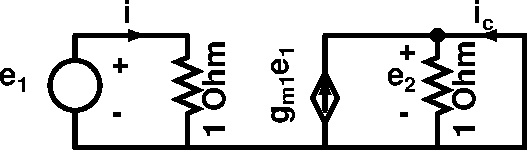
\includegraphics[totalheight=.2\textheight,width=.6\textwidth]{images/ex3c}}
\caption{State variable=0}
\label{ex3c}
\end{figure}

\item Step 6: Calculate $I_c$ in terms of input voltage $e_1$.
\begin{equation}
I_c=-g_{m1}e_1=-e_1; \hspace{0.2in}C\dot{V}_c =-e_1;\hspace{0.2in} \dot{V}_c =-\frac{1}{C}e_1;\hspace{0.2in}[B]=-\frac{1}{C}=-1
\end{equation}
         \end{itemize}
\end{small}
\end{frame}

%%%%%%%%%%%%%%%%%%%%%%%%% 1000
%%%%%%%%%%%%%%%%%%%%%%%%% 1000
%%%%%%%%%%%\section{Compensation Design Example}
\subsection*{Example}

\begin{frame}
\frametitle{Example}
\begin{small}

        \begin{itemize}
% \begin{itemize}
\item Step 7: Determine the output i, in terms of input $e_1$.
\begin{equation}
i=e_{1};\hspace{0.2in}[D]=1
\end{equation} 
         
\item Hence State Space Representation of the circuit shown in Fig.\ref{ex3a}.\\
\begin{equation}
 \dot{V_c}=[1][V_c]+[-1][e_1];\hspace{0.2in}[i]=[-2][V_c]+[1][e_1]
\end{equation}
\item Controllablity and Observablity matrix are as:\\

 $C_o$=[B]=[-1] $\neq$ 0 and $Q_o=[C^T]$=[-2]$\neq 0$, respectively \\

therefore system is controllable, as well as Observable. 
\item As the Eigen values of matrix A is +1, i.e. pole of $Z_{in}$ lie is RHS of s plane therefore, system is Open circuit unstable.
\end{itemize}
\end{small}
\end{frame}




%%%%%%%%%%%%%%%%%%%%%%%%% 1000
%%%%%%%%%%%%%%%%%%%%%%%%% 1000
%%%%%%%%%%%\section{Compensation Design Example}
\subsection*{Example}

\begin{frame}
\frametitle{Example}
\begin{small}

        \begin{itemize}
% \begin{itemize}
\item Now we will make the compensator by state space approach\cite{Chua}
\item {\bf{Step 1:}} A, B, C, D for the given network are:\\
A=1, B=-1, C=-2, D=1
\item {\bf{Step 2:}} Coprime factorization of Z(s) can be done so as to get four rational functions N(s),D(s), X(s) and Y(s) \cite{Chua}, all in $\wp$, such that Z(s)=$ \frac{N(s)}{D(s)} $\\
N(s)X(s)+D(s)Y(s)=1

\begin{itemize}
      \item Calculation of N(s), D(s): Choose a real matrix F = $[f_1]$, $ 1\times 1$, such that $A + BF$ is stable i.e. all the eigenvalues in Re s$<$0. Let the eigenvalue of A + BF be located at -1. The desired characteristics equation is (s+1).\\
                $|sI-(A+BF)| =|s(1)-(1+(-1)f_1|=s+(-1+f_1)$\\
Comparing coefficients of above equation with those of desired equation we get, $f_1=2$ thus F=[2].

 \end{itemize}
\end{itemize}
\end{small}
\let\thefootnote\relax\footnotetext[\value{footnote}]{\tiny{{{~\cite{Chua}\color{blue}L.O.Chua, C.A.Deoser and E.H.Kuh, Linear and Nonlinear Circuits. New York: Mcgraw-Hill,1987}}}}
\end{frame}





%%%%%%%%%%%%%%%%%%%%%%%%% 1000
%%%%%%%%%%%%%%%%%%%%%%%%% 1000
%%%%%%%%%%%\section{Compensation Design Example}
\subsection*{Example}

\begin{frame}
\frametitle{Example}
\begin{small}

        \begin{itemize}
% \begin{itemize}
\item The transfer function from v to u is given by,\\
 $D(s)=1+F[sI-(A+BF)]^{-1}B)$ which can be represent as
\[ \left[ \begin{array}{c|c}
A+BF& B \\
\hline
F & 1 \end{array} \right].\]
\begin{equation}
D(s)=\frac{s-1}{s+1}
\end{equation}
\item The transfer from v to y is given by,\\
 $N(s)=D+(C+DF)[sI-(A+BF)]^{-1}B)$  which can be represent as 
\[ \left[ \begin{array}{c|c}
A+BF& B \\
\hline
C+DF & D \end{array} \right]\]
\begin{equation}
N(s)=1
\end{equation}
\end{itemize}
\end{small}

\end{frame}


%%%%%%%%%%%%%%%%%%%%%%%%%%%%%%%%%%%%%%%%%







%%%%%%%%%%%%%%%%%%%%%%%%% 1000
%%%%%%%%%%%%%%%%%%%%%%%%% 1000
%%%%%%%%%%%\section{Compensation Design Example}
%%%%%%%%%%%%%%%%%%%%%%%%% 1000
%%%%%%%%%%%%%%%%%%%%%%%%% 1000
%%%%%%%%%%%\section{Compensation Design Example}


%%%%%%%%%%%%%%%%%%%%%%%%% 1000
%%%%%%%%%%%%%%%%%%%%%%%%% 1000
%%%%%%%%%%%\section{Compensation Design Example}
\subsection*{Example}

\begin{frame}
\frametitle{Example}
\begin{small}

        \begin{itemize}
% \begin{itemize}
      \item Calculation of X(s), Y(s).Choose a real matrix H = $[h_1]$, $ 1 \times 1$, such that $A + HC$ is stable i.e. all the eigenvalues in Re s$<$0. Let the eigenvalue of A + BF be located at -1. The desired characteristics equation is (s+1).\\
               $|sI-(A+HC)| =|s(1)-(1+(-2)h_1|=s+(-1+h_1(-2))$\\
Comparing coefficients of above equation with those of desired equation we get, $h_1=1$ thus H=[1].\\
\item The transfer function from v to u is given by,\\
 $X(s)=F[sI-(A+HC)]^{-1}H)$ which can be represent as 
\[ \left[ \begin{array}{c|c}
A+HC& H \\
\hline
F & 0 \end{array} \right]\] 
\begin{equation}
X(s)=\frac{2}{s+1}
\end{equation}
  %\end{itemize}
\end{itemize}
\end{small}
\end{frame}





%%%%%%%%%%%%%%%%%%%%%%%%% 1000
%%%%%%%%%%%%%%%%%%%%%%%%% 1000
%%%%%%%%%%%\section{Compensation Design Example}
\subsection*{Example}

\begin{frame}
\frametitle{Example}
\begin{small}

        \begin{itemize}
% \begin{itemize}
\item The transfer from v to y is given by,\\
 $Y(s)=1+F[sI-(A+HC)]^{-1}(-B-HD)$  which can be represent as 
\[ \left[ \begin{array}{c|c}
A+HC& -B-HD \\
\hline
F & 1 \end{array} \right]\]  
\begin{equation}
Y(s)=1
\end{equation}
\item Thus we have following four rational function satisfying Bezout's identity\\ \begin{equation}
N(s)=1;\hspace{0.2in} D(s)=\frac{s-1}{s+1};\hspace{0.2in} X(s)=\frac{2}{s+1};\hspace{0.2in} Y(s)=1
\end{equation}
\end{itemize}
\end{small}

\end{frame}




%%%%%%%%%%%%%%%%%%%%%%%%% 1000
%%%%%%%%%%%%%%%%%%%%%%%%% 1000
%%%%%%%%%%%\section{Compensation Design Example}
\subsection*{Example}

\begin{frame}
\frametitle{Example}
\begin{small}

        \begin{itemize}
% \begin{itemize}
\item The compensator transfer function is given as:
\begin{equation}
Z_c =\frac{Y(s)-N(s)Q(s)}{X(s)+D(s)Q(s)}
\end{equation}
where Q(S) is free parameter $\in \wp$\\
Let us assune, Q=0.5, then $Z_c$ is given as,
\begin{equation}
Z_c =\frac{(s+1)}{(s+3)}
\end{equation}
\item Total impedance after connecting the compensator is $Z_T$=N(s)[Y(s)-N(s)Q]=1[1-(0.5)1]=0.5\\
Hence Overall system after connecting the compensator become stable.

\end{itemize}
\end{small}

\end{frame}






%%%%%%%%%%%%%%%%%%%%%%%%% 1000
%%%%%%%%%%%%%%%%%%%%%%%%% 1000
%%%%%%%%%%%\section{Compensation Design Example}
\subsection*{state space}

\begin{frame}
\frametitle{Example}

\begin{small}
        \begin{itemize}
	\item Same example is simulated in the Scilab code, Bode Plot obtain is shown in Fig.\ref{be}:
\begin{figure}[h!]
\centering
{\label{method}\includegraphics[scale=0.3]{images/bodeEX.png}}
%\subfloat[]{\label{mlfsr}\includegraphics[totalheight=.3\textheight,width=.3\textwidth]{images/LowFreqMag.png}}
\caption{Bode Plot from Scilab Code}
\label{be}
\end{figure} 

         \end{itemize}
\end{small}


\end{frame}



%%%%%%%%%%%%%%%%%%%%%%%%% 11

\section{Conclusion}
\subsection*{Formulation}

\begin{frame}
\frametitle{Conclusion}

\begin{small}
        \begin{itemize}
 \item Stabilization problem for one port networks has been studied and solved.
\item The set of compensating networks depending on the Q free parameter which will stabilize the given one port network can be obtained by the application of coprime factorization theory via state space realization of the networks. 
\item Finding the state space representation of given network by method discussed has certain limitation
\item The network should not have node with the only elements incident at node comprising inductor and/or current generator i.e the network should contain a cut set.The network does not contain a loop with the only branches in the loop comprising capacitor and/or voltage generator. i.e. the network does not have a tie set.

        \end{itemize}
\end{small}
\end{frame}

%%%%%%%%%%%%%%%%%%%%%%%%% 11

\subsection*{Formulation}

\begin{frame}
\frametitle{Future Work}

\begin{small}
        \begin{itemize}
 \item Solving the stabilization problem for two port networks.
 \item Applying coprime factorization approach to multivariate system and to obtain set of compensating networks.
 \item Synthesis the compensator network. 
 \item Applying the algorithm to find state space with simulator, and try to find state space for more practical case without any limitation.
%%% \item Solving problems of two port networks to illustrate the application of the concepts developed to physical networks.
 \item Application of these concepts to practical circuits such as multistage amplifiers to design a suitable compensator and to evaluate its performance with various process technology.
        \end{itemize}
\end{small}
\end{frame}





\section{Bibliography}
\removepagenumbers{
\begin{frame}
\addtocounter{framenumber}{-1}
	\frametitle{Bibliography:}
\tiny
\begin{thebibliography}{50}
\addtolength{\leftmargin}{0.2in} % sets up alignment with the following line.
\setlength{\itemindent}{-0.2in}

\bibitem{Haykin}
S.S.Haykin, Active Network Theory, Addison-Wesley Publishing Company, 1970.

\bibitem{Doyle}
John C. Doyle and Keith Glover, Robust and Optimal Control, Prentice Hall, New Jersey 1996.

\bibitem{Deoser} 
C.A.Deoser, R.W.Liu, John Murray and Richard Sakes, “Feedback System Design: The Fractional Representation Approach to Analysis and Synthesis, IEEE Trans. on Automatic Control, Vol.AC-25, No.3, pp 399-412, June 1980.

\bibitem{Vidya}
M.Vidyasagar, Control System Synthesis: a Factorization Approach, Cambridge: MIT Press, 1985.

\bibitem{Bhatt}
S.P.Bhattacharyya,  A.Datta, L.H.Keel, Linear Control Theory Structure Robustness and Optimization, Boca Rotan: CRC press, 2009.

\bibitem{DoyleF}
John C. Doyle, Bruce A. Francis, Allen R. Tannenbaum, Feedback Control Theory, Dover Publications, Inc. Mineola, New York, 2009.


\bibitem{Chua}
L.O.Chua, C.A.Deoser and E.H.Kuh, Linear and Nonlinear Circuits. New York: Mcgraw-Hill,1987


\bibitem{LC00}
P.Dorato, L.Fortuna, G.Muscato, Lecture Notes in Control and Information Sciences: Robust Control for Unstructured Perturbations – An Introduction, Edited by M.Thoma and A Wyner,Springer-Verlag, 1992. 

\bibitem{Mitra}
Sanjit Kumar Mitra, Analysis and Synthesis of Linear Active Networks, John Wiley and Sons, Inc,1969.

\bibitem{Razavi} 
B. Razavi, Design of analog CMOS integrated circuits, McGraw-Hill Book Edition,
2005.

\bibitem{Cadence} 
C.S.U. Manual, “Cadence design systems,” San Jose, CA, 1994.

\bibitem{Scilab} 
Scilab Consortium et al., “Scilab manual,” 2010.

\bibitem{Manu}
 C. G ́mez, Engineering and scientific computing with scilab, Birkhauser, 1999.


\end{thebibliography}
\end{frame}

%%%%%%%%%%%%%%%%%%%5555
\begin{frame}
\addtocounter{framenumber}{-1}
	\frametitle{Bibliography:}
\tiny
\begin{thebibliography}{50}
\addtolength{\leftmargin}{0.2in} % sets up alignment with the following line.
\setlength{\itemindent}{-0.2in}


\bibitem{Doy} K. Zhou, J.C. Doyle, K. Glover, et al., Robust and optimal control, vol. 40, Prentice
Hall Upper Saddle River, NJ, 1996.

\bibitem{Ander} 
B.D.O. Anderson and S. Vongpanitlerd, Network analysis and synthesis: a modern
systems theory approach, Courier Dover Publications, 2006.

\bibitem{Marin}T. Martinez-Marin, “State-space formulation for circuit analysis,” Education, IEEE
Transactions on, vol. 53, no. 3, pp. 497–503, 2010.

\bibitem{statespace}
D.C. Karamousantas, G.E. Chatzarakis, G.N. Korres, and P.J. Katsikas, “Obtaining
state equations for planar nondegenerate linear electric circuits using mesh analysis
with virtual voltage sources,” International Journal of Electrical Engineering Educa-
tion, vol. 45, no. 3, pp. 239–250, 2008.

\bibitem{StateNat}
S. Natarajan, “A systematic method for obtaining state equations using mna,” in
Circuits, Devices and Systems, IEE Proceedings G. IET, 1991, vol. 138, pp. 341–346.

\bibitem{ss}
D.L. Skaar, “Using the superposition method to formulate the state variable matrix
for linear networks,” Education, IEEE Transactions on, vol. 44, no. 4, pp. 311–314,
2001.




\end{thebibliography}
\end{frame}
\addtocounter{framenumber}{-1}
\section*{}
\subsection*{}
\begin{frame}
	\begin{block}{\Large \bf {Thank You}}
	\end{block}
\end{frame}

\end{document}

%%%%%%%%%%%%%%%%%%%%%%%%%%%%%%%%%%%%%%%%%%%%%%%%%%%%%%%%%%%%%%%%%%%%%%%%%%%%%%%%%%%%%%%%%%%%%%%%%%%%%%%%%%%%%%%%


